\begin{frame}[parent={ie:agenda}, hasnext=false, hasprev=false]
	\frametitle{Qualidade de produto}
	
	\begin{block:concept}{Qualidade de produto}
		Qualidade é a totalidade de características e critérios de um produto ou
		serviço que exercem suas habilidades para satisfazer as necessidades 
		declaradas ou envolvidas.
	\end{block:concept}
	
	\begin{block:fact}{}
		Embora seja difícil definir exatamente qualidade (em termos de satisfação
		de propriedades), é fácil reconhecer produtos de boa qualidade.
	\end{block:fact}
\end{frame}


\begin{frame}[hasnext=true, hasprev=true]
	\frametitle{Qualidade de produto}
	
	\begin{block:fact}{Qualidade de produto e processo}
		\centering
		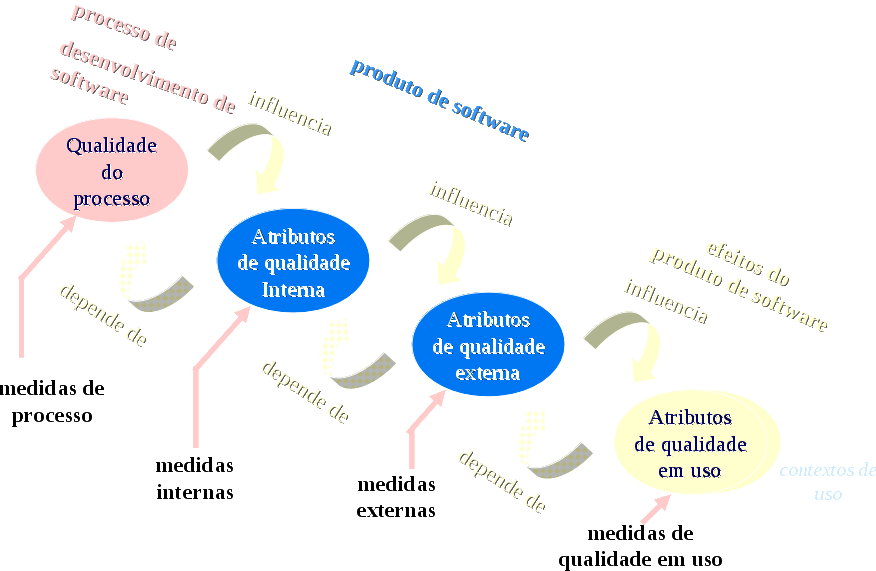
\includegraphics[width=\textwidth]{software-engineering/project-management/product/product-quality}
	\end{block:fact}
	
	\begin{block:fact}{}
		A avaliação de produtos de software tem sido uma das formas empregadas por
		organizações que produzem ou adquirem software para obtenção de maior
		qualidade nesses produtos, sejam eles produtos completos ou partes a serem
		integradas num sistema computacional mais amplo.
	\end{block:fact}
\end{frame}


\begin{frame}
	\frametitle{Qualidade de produto}
	
	\begin{block:fact}{Perspectivas}
		\centering
		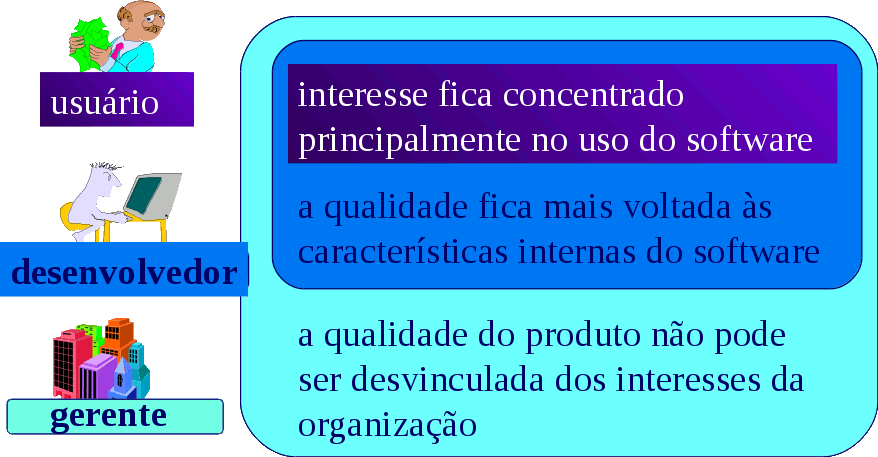
\includegraphics[width=\textwidth]{software-engineering/project-management/product/product-quality-perspectives}
	\end{block:fact}
\end{frame}


\begin{frame}
	\frametitle{Qualidade de produto}
	\framesubtitle{Modelos de qualidade}
	
	\begin{block:fact}{Modelos de qualidade de produto}
		\begin{itemize}
			\item Modelo de McCall
			\item Modelo de qualidade da ISO 9126
			\item Modelo de Dromey
			\item Modelo da 25010
		\end{itemize}
	\end{block:fact}
\end{frame}


